%%%%%%%%%%%%%%%%%%%%%%%%%%%%%%%%%%%%%%%%%%%%%%%%%%%%%%%%%%%%%%%%%%%%%%
%%  Copyright by Wenliang Du.                                       %%
%%  This work is licensed under the Creative Commons                %%
%%  Attribution-NonCommercial-ShareAlike 4.0 International License. %%
%%  To view a copy of this license, visit                           %%
%%  http://creativecommons.org/licenses/by-nc-sa/4.0/.              %%
%%%%%%%%%%%%%%%%%%%%%%%%%%%%%%%%%%%%%%%%%%%%%%%%%%%%%%%%%%%%%%%%%%%%%%

\newcommand{\commonfolder}{../../common-files}
\newcommand{\webcommon}{../Web_Common}

\documentclass[11pt]{article}

\usepackage[most]{tcolorbox}
\usepackage{times}
\usepackage{epsf}
\usepackage{epsfig}
\usepackage{amsmath, alltt, amssymb, xspace}
\usepackage{wrapfig}
\usepackage{fancyhdr}
\usepackage{url}
\usepackage{verbatim}
\usepackage{fancyvrb}
\usepackage{adjustbox}
\usepackage{listings}
\usepackage{color}
\usepackage{subfigure}
\usepackage{cite}
\usepackage{sidecap}
\usepackage{pifont}
\usepackage{mdframed}
\usepackage{textcomp}
\usepackage{enumitem}


% Horizontal alignment
\topmargin      -0.50in  % distance to headers
\oddsidemargin  0.0in
\evensidemargin 0.0in
\textwidth      6.5in
\textheight     8.9in 

\newcommand{\todo}[1]{
\vspace{0.1in}
\fbox{\parbox{6in}{TODO: #1}}
\vspace{0.1in}
}


\newcommand{\unix}{{\tt Unix}\xspace}
\newcommand{\linux}{{\tt Linux}\xspace}
\newcommand{\minix}{{\tt Minix}\xspace}
\newcommand{\ubuntu}{{\tt Ubuntu}\xspace}
\newcommand{\setuid}{{\tt Set-UID}\xspace}
\newcommand{\openssl} {\texttt{openssl}}


\pagestyle{fancy}
\lhead{\bfseries SEED Labs}
\chead{}
\rhead{\small \thepage}
\lfoot{}
\cfoot{}
\rfoot{}


\definecolor{dkgreen}{rgb}{0,0.6,0}
\definecolor{gray}{rgb}{0.5,0.5,0.5}
\definecolor{mauve}{rgb}{0.58,0,0.82}
\definecolor{lightgray}{gray}{0.90}


\lstset{%
  frame=none,
  language=,
  backgroundcolor=\color{lightgray},
  aboveskip=3mm,
  belowskip=3mm,
  showstringspaces=false,
%  columns=flexible,
  basicstyle={\small\ttfamily},
  numbers=none,
  numberstyle=\tiny\color{gray},
  keywordstyle=\color{blue},
  commentstyle=\color{dkgreen},
  stringstyle=\color{mauve},
  breaklines=true,
  breakatwhitespace=true,
  tabsize=3,
  columns=fullflexible,
  keepspaces=true,
  escapeinside={(*@}{@*)}
}

\newcommand{\newnote}[1]{
\vspace{0.1in}
\noindent
\fbox{\parbox{1.0\textwidth}{\textbf{Note:} #1}}
%\vspace{0.1in}
}


%% Submission
\newcommand{\seedsubmission}{You need to submit a detailed lab report, with screenshots,
to describe what you have done and what you have observed.
You also need to provide explanation
to the observations that are interesting or surprising.
Please also list the important code snippets followed by
explanation. Simply attaching code without any explanation will not
receive credits.}

%% Book
\newcommand{\seedbook}{\textit{Computer \& Internet Security: A Hands-on Approach}, 2nd
Edition, by Wenliang Du. See details at \url{https://www.handsonsecurity.net}.}

%% Videos
\newcommand{\seedisvideo}{\textit{Internet Security: A Hands-on Approach},
by Wenliang Du. See details at \url{https://www.handsonsecurity.net/video.html}.}

\newcommand{\seedcsvideo}{\textit{Computer Security: A Hands-on Approach},
by Wenliang Du. See details at \url{https://www.handsonsecurity.net/video.html}.}

%% Lab Environment
\newcommand{\seedenvironment}{This lab has been tested on our pre-built
Ubuntu 16.04 VM, which can be downloaded from the SEED website. }

\newcommand{\seedenvironmentA}{This lab has been tested on our pre-built
Ubuntu 16.04 VM, which can be downloaded from the SEED website. }

\newcommand{\seedenvironmentB}{This lab has been tested on our pre-built
Ubuntu 20.04 VM, which can be downloaded from the SEED website. }

\newcommand{\seedenvironmentAB}{This lab has been tested on our pre-built
Ubuntu 16.04 and 20.04 VMs, which can be downloaded from the SEED website. }

\newcommand{\nodependency}{Since we use containers to set up the lab environment, 
this lab does not depend too much on our SEED VM. You can do this lab
using other VMs or physical machines. }







\newcommand{\seedlabcopyright}[1]{
\vspace{0.1in}
\fbox{\parbox{6in}{\small Copyright \copyright\ {#1}\ \ by Wenliang Du.\\
      This work is licensed under a Creative Commons
      Attribution-NonCommercial-ShareAlike 4.0 International License.
      If you remix, transform, or build upon the material, 
      this copyright notice must be left intact, or reproduced in a way that is reasonable to
      the medium in which the work is being re-published.}}
\vspace{0.1in}
}







\lhead{\bfseries SEED Labs -- SQL Injection Attack Lab}

\newcommand{\sqlFigs}{./Figs}


\begin{document}


\begin{center}
{\LARGE SQL Injection Attack Lab }
\end{center}

\seedlabcopyright{2006 - 2020}


% *******************************************
% SECTION
% ******************************************* 
\section{Overview}

SQL injection is a code injection technique that exploits the 
vulnerabilities in the interface between web applications and 
database servers. The vulnerability is present when user's inputs 
are not correctly checked within the web applications 
before being sent to the back-end database servers.

Many web applications take inputs from users, and then use these
inputs to construct SQL queries, so they can get information from the database.
Web applications also use SQL queries to store information in
the database. These are common practices in the development of web applications.
When SQL queries are not carefully constructed, 
SQL injection vulnerabilities can occur. 
SQL injection is one of the most common 
attacks on web applications.


In this lab, we have created a web application that is vulnerable to the SQL injection attack. 
Our web application includes the common mistakes made by many web developers. 
Students' goal is to find ways to exploit the SQL injection vulnerabilities,
demonstrate the damage that can be achieved by the attack, 
and master the techniques that can help defend against such type of attacks.
This lab covers the following topics:

\begin{itemize}[noitemsep]
\item SQL statements: \texttt{SELECT} and \texttt{UPDATE} statements
\item SQL injection
\item Prepared statement
\end{itemize}



\paragraph{Readings.}
Detailed coverage of the SQL injection can be found in the following:

\begin{itemize}
\item Chapter 12 of the SEED Book, \seedbook
\end{itemize}

\paragraph{Lab Environment.} \seedenvironmentB \nodependency
You do need to add the required IP address mapping to
the \texttt{/etc/hosts} file.  


% *******************************************
% SECTION
% ******************************************* 
\section{Lab Environment}


We have developed a web application for this lab. It is 
accessible via \url{http://www.SEEDLabSQLInjection.com}. 
We use containers to set up this web application. There 
are two containers in the lab setup, one for hosting 
the web application, and the other for hosting the database 
for the web application. 
The IP address for the web application container is \texttt{10.9.0.5}, and 
the mapping between the URL and the IP address is 
already added to the \texttt{/etch/hosts} file in the 
SEED VM. If you are not using the SEED VM, you
need to add this mapping to your system. 


% -------------------------------------------
% SUBSECTION
% -------------------------------------------
\subsection{Container Setup and Commands}

%%%%%%%%%%%%%%%%%%%%%%%%%%%%%%%%%%%%%%%%%%%%
Please download the
\texttt{Labsetup.zip} file to your VM from the lab's website,
unzip it, enter the \texttt{Labsetup} folder, and 
use the \texttt{docker-compose.yml} file to 
set up the lab environment. Detailed explanation
of the content in this file and all the involved 
\texttt{Dockerfile} can be found from the 
user manual, which is linked to the website of this lab.
If this is the first time you set up a SEED lab environment
using containers, it is very important that you read 
the user manual. 

In the following, we list some of the commonly
used commands related to Docker and Compose. 
Since we are going to use 
these commands very frequently, we have created aliases for them
in the \texttt{.bashrc} file (in our provided SEEDUbuntu 20.04 VM).


\begin{lstlisting}
$ docker-compose build  # Build the container image
$ docker-compose up     # Start the container
$ docker-compose down   # Shut down the container

// Aliases for the Compose commands above
$ dcbuild       # Alias for: docker-compose build
$ dcup          # Alias for: docker-compose up
$ dcdown        # Alias for: docker-compose down
\end{lstlisting}


All the containers will be running in the background. To run
commands on a container, we often need to get a shell on
that container. We first need to use the \texttt{"docker ps"}  
command to find out the ID of the container, and then
use \texttt{"docker exec"} to start a shell on that 
container. We have created aliases for them in
the \texttt{.bashrc} file.

\begin{lstlisting}
$ dockps        # Alias for: docker ps --format "{{.ID}}  {{.Names}}" 
$ docksh <id>   # Alias for: docker exec -it <id> /bin/bash

# The following example shows how to get a shell inside hostC
$ dockps
b1004832e275  hostA-10.9.0.5
0af4ea7a3e2e  hostB-10.9.0.6
9652715c8e0a  hostC-10.9.0.7

$ docksh 96
root@9652715c8e0a:/#  

# Note: If a docker command requires a container ID, you do not need to 
#       type the entire ID string. Typing the first few characters will 
#       be sufficient, as long as they are unique among all the containers. 
\end{lstlisting}


If you encounter problems when setting up the lab environment, 
please read the ``Common Problems'' section of the manual
for potential solutions.


%%%%%%%%%%%%%%%%%%%%%%%%%%%%%%%%%%%%%%%%%%%%


% MySQL database
%%%%%%%%%%%%%%%%%%%%%%%%%%%%%%%%%%%%

\paragraph{MySQL database.}
Containers are usually disposable, so once it
is destroyed, all the data inside the containers are lost.
For this lab, we do want to keep the data in the
MySQL database, so we do not lose our work when we shutdown
our container. To achieve this,
we have mounted the \texttt{mysql\_data} folder on
the host machine (inside
\texttt{Labsetup}, it will be created after the
MySQL container runs once) to the
\texttt{/var/lib/mysql} folder
inside the MySQL container.
This folder is where
MySQL stores its database. Therefore,
even if the container is destroyed,
data in the database are still kept.
If you do want to start from a clean
database, you can remove this folder:

\begin{lstlisting}
$ sudo rm -rf mysql_data
\end{lstlisting}


%%%%%%%%%%%%%%%%%%%%%%%%%%%%%%%%%%%%



% -------------------------------------------
% SUBSECTION
% -------------------------------------------
\subsection{About the Web Application} 

We have created a web application, which is a simple employee 
management application. 
Employees can view and update their personal information 
in the database through this web application. 
There are mainly two roles in this web application: 
{\tt Administrator} is a privilege role and can manage each individual
employees' profile information;
{\tt Employee} is a normal role and can view or update his/her own profile 
information. All employee information is described in Table~\ref{table:database}.


\begin{table}[htb]
\caption{Database}
\label{table:database}
\centering
\begin{adjustbox}{max width=\textwidth}
\begin{tabular}{|l|l|l|l|l|l|l|l|l|l|l|}
\hline
Name & Employee ID  & Password  &Salary  &Birthday  &SSN &Nickname &Email &Address &Phone\# \\
\hline
Admin 	& 99999       & seedadmin  &400000  &3/5   &43254314	& & & &\\
Alice 	& 10000       & seedalice  &20000   &9/20  &10211002	& & & &\\
Boby 	& 20000       & seedboby   &50000   &4/20  &10213352	& & & &\\
Ryan    & 30000       & seedryan   &90000   &4/10  &32193525	& & & &\\
Samy 	& 40000	      & seedsamy   &40000   &1/11  &32111111 	& & & &\\
Ted     & 50000	      & seedted    &110000  &11/3  &24343244	& & & &\\
\hline
\end{tabular}
\end{adjustbox}
\end{table}
 



% *******************************************
% SECTION
% ******************************************* 
\section{Lab Tasks}



% -------------------------------------------
% SUBSECTION
% ------------------------------------------- 
\subsection{Task 1: Get Familiar with SQL Statements}
\label{ssec:MySQLConsole}


The objective of this task is to get familiar with SQL commands by playing
with the provided database. The data used by our web application
is stored in a MySQL database, which is hosted on our 
MySQL container. 
We have created a database called \texttt{sqllab\_users},
which contains a table called {\tt credential}. The table stores
the personal information (e.g. eid, password, salary, ssn, etc.) of every
employee. In this task, you need to play with the database to get familiar
with SQL queries.

Please get a shell on the MySQL container (see the container manual for 
instruction; the manual is linked to the lab's website).
Then use the \texttt{mysql} client program to 
interact with the database. 
The user name is {\tt root} and password is {\tt dees}.  

	
\begin{lstlisting}
// Inside the MySQL container
# mysql -u root -pdees 
\end{lstlisting}


After login, you can create new database or load an existing
one. As we have already created the \texttt{sqllab\_users} database for you, you just
need to load this existing database using the \texttt{use} command. 
To show what tables are there in the \texttt{sqllab\_users} database, 
you can use the \texttt{show tables} command to print out all the tables of the
selected database.

\begin{lstlisting}
mysql> use sqllab_users;
Database changed
mysql> show tables;
+------------------------+
| Tables_in_sqllab_users |
+------------------------+
| credential             |
+------------------------+
\end{lstlisting}


After running the commands above, you need to use 
a SQL command to print all the profile information of
the employee Alice. Please provide the screenshot of your results.


% -------------------------------------------
% SUBSECTION
% ------------------------------------------- 
\subsection{Task 2: SQL Injection Attack on SELECT Statement} 


SQL injection is basically a technique through
which attackers can execute their own malicious SQL statements generally
referred as malicious payload. Through the malicious SQL statements, 
attackers can steal information from the victim database; even worse,
they may be able to make changes to the database. Our employee
management web application has SQL injection vulnerabilities, which mimic 
the mistakes frequently made by developers. 

We will use the login page from \url{www.SEEDLabSQLInjection.com}
for this task. The login page is shown in Figure~\ref{sql:fig:login}. 
It asks users to provide a user name and a password.
The web application authenticate users based on these two pieces 
of data, so only employees who know their 
passwords are allowed to log in.
Your job, as an attacker, is to log into the web application without knowing
any employee's credential. 


\begin{figure}[htb]
\begin{center}
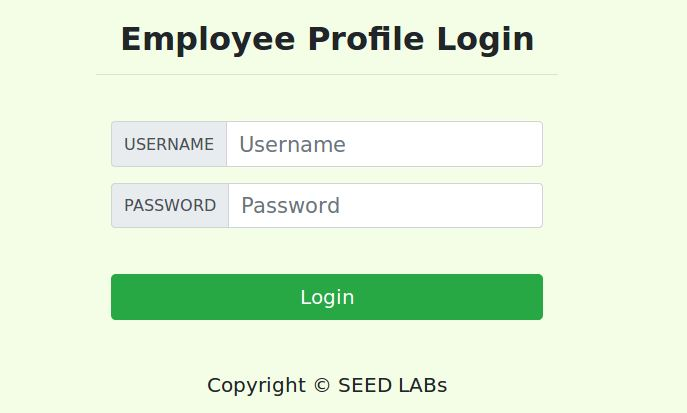
\includegraphics[width=0.7\textwidth]{\sqlFigs/login.jpg}
\end{center}
\caption{The Login page}
\label{sql:fig:login}
\end{figure}
 

To help you started with this task, we explain how authentication
is implemented in the web application. The PHP code 
\texttt{unsafe\_home.php}, located in the \path{/var/www/SQL_Injection} directory, 
is used to conduct user authentication.
The following code snippet show how users are authenticated. 

\begin{lstlisting}
$input_uname = $_GET['username'];
$input_pwd = $_GET['Password'];
$hashed_pwd = sha1($input_pwd);
...
$sql = "SELECT id, name, eid, salary, birth, ssn, address, email, 
               nickname, Password
        FROM credential
        WHERE name= '$input_uname' and Password='$hashed_pwd'";
$result = $conn -> query($sql);

// The following is Pseudo Code 
if(id != NULL) {
  if(name=='admin') {
     return All employees information;
  } else if (name !=NULL){
    return employee information;
  }
} else {
  Authentication Fails;
}
\end{lstlisting}

The above SQL statement selects personal employee information such as id,
name, salary, ssn etc from the {\tt credential} table. The SQL statement
uses two variables \texttt{input\_uname} and \texttt{hashed\_pwd},
where \texttt{input\_uname} holds the string typed by 
users in the username field of the login page, while 
\texttt{hashed\_pwd} holds the \texttt{sha1} hash of the password typed by
the user. The program checks whether 
any record matches with the provided username and password; if there is a match,
the user is successfully authenticated, and is given the corresponding 
employee information. If there is no match, the authentication
fails. 



\paragraph{Task 2.1: SQL Injection Attack from webpage.}
Your task is to log into the web application as 
the administrator from the login page, so you can see the information of
all the employees. We assume that you do know the administrator's account name
which is {\tt admin}, but you do not the password. You need to decide
what to type in the \texttt{Username} and \texttt{Password} fields to
succeed in the attack.
	


\paragraph{Task 2.2: SQL Injection Attack from command line.}  
Your task is to repeat Task 2.1, but you need to do it without 
using the webpage. You can use command line tools, such as 
\texttt{curl}, which can send HTTP requests. 
One thing that is worth mentioning is that if you
want to include multiple parameters in HTTP requests, you need to put the
URL and the parameters between a pair of single quotes; otherwise, the 
special characters used to separate parameters (such as \texttt{\&}) will be
interpreted by the shell program, changing the meaning of the 
command. The following example shows how to send an HTTP GET request to our 
web application, with two parameters (\texttt{username} and 
\texttt{Password}) attached:

\begin{lstlisting}
$ curl 
 'www.SeedLabSQLInjection.com/unsafe_home.php?username=alice&Password=11'
\end{lstlisting}

If you need to include special characters in the 
\texttt{username} or \texttt{Password} fields, you need to 
encode them properly, or they can change the meaning of your 
requests. If you want to include single quote in those fields,
you should use \texttt{\%27} instead; if you want to include
white space, you should use \texttt{\%20}. In this
task, you do need to handle HTTP encoding while sending
requests using \texttt{curl}.



\paragraph{Task 2.3: Append a new SQL statement.}  
In the above two attacks, we can only steal information from the database;
it will be better if we can modify the database using the same
vulnerability in the login page.  An idea is to use the SQL injection
attack to turn one SQL statement into two, with the second one being the
update or delete statement. In SQL, semicolon (;) is used to separate two SQL
statements. Please try to run two SQL statements via the login page. 

There is a countermeasure preventing you from running two
SQL statements in this attack. Please use the SEED book 
or resources from the Internet to figure out what this 
countermeasure is, and describe your discovery in the lab report. 



% -------------------------------------------
% SUBSECTION
% ------------------------------------------- 
\subsection{Task 3: SQL Injection Attack on UPDATE Statement} 

If a SQL injection vulnerability happens to an UPDATE statement, the damage will be more
severe, because attackers can use the vulnerability to modify databases. 
In our Employee Management application, there is an Edit Profile page~(Figure~\ref{sql:fig:edit}) 
that allows employees to
update their profile information, including nickname, email, address, phone number, and
password. To go to this page, employees need to log in first. 


When employees update their information through the Edit Profile page, the
following SQL UPDATE query will be executed. The PHP code implemented in
{\tt unsafe\_edit\_backend.php} file is used to update employee's profile
information. The PHP file is located in the {\tt /var/www/SQLInjection}
directory.


\begin{lstlisting}
$hashed_pwd = sha1($input_pwd);
$sql = "UPDATE credential SET
	nickname='$input_nickname',
	email='$input_email',
	address='$input_address',
	Password='$hashed_pwd',
	PhoneNumber='$input_phonenumber'
	WHERE ID=$id;";
$conn->query($sql);
\end{lstlisting}
 

\begin{figure}[htb]
\begin{center}
  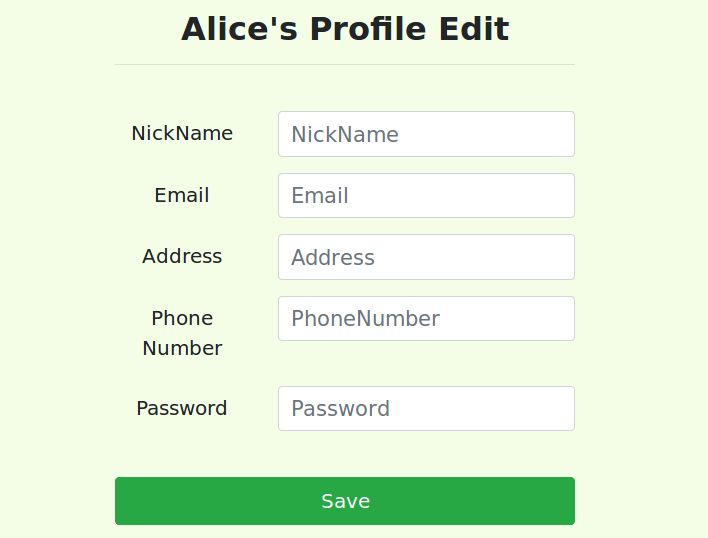
\includegraphics[width=0.6\textwidth]{\sqlFigs/editprofile.jpg}
\end{center}
\caption{The Edit-Profile page}
\label{sql:fig:edit}
\end{figure}
 


\paragraph{Task 3.1: Modify your own salary.}  
As shown in the Edit Profile page,
employees can only update their nicknames, emails, addresses, phone numbers, and
passwords; they are not authorized to change their salaries.  
Assume that you (Alice) are a disgruntled employee, and your boss Boby did not 
increase your salary this year. You want to increase your own salary 
by exploiting the SQL injection vulnerability in
the Edit-Profile page. Please demonstrate how you can achieve that.
We assume that you do know that salaries are stored in 
a column called \texttt{salary}.


\paragraph{Task 3.2: Modify other people' salary.}
After increasing your own salary, you decide to punish your boss Boby. You want to reduce his
salary to 1 dollar. Please demonstrate how you can achieve that. 



\paragraph{Task 3.3: Modify other people' password.}
After changing Boby's salary, you are still disgruntled, so you
want to change Boby's password to something that you know, and then you can log into his account
and do further damage. Please demonstrate how you can achieve that.
You need to demonstrate that you can 
successfully log into Boby's account using the new
password.  One thing worth mentioning here is that the database stores the hash value of
passwords instead of the plaintext password string. You can again look at
the {\tt unsafe\_edit\_backend.php} code to see how password is being stored. It
uses SHA1 hash function to generate the hash value of password. 




\subsection{Task 4: Countermeasure --- Prepared Statement} 

The fundamental problem of the SQL injection vulnerability is the failure to
separate code from data. When constructing a SQL statement, the program
(e.g. PHP program) knows which part is data and which part is code.
Unfortunately, when the SQL statement is sent to the database, the boundary
has disappeared; the boundaries that the SQL interpreter sees may be
different from the original boundaries that was set by the developers.
To solve this problem, it is important to ensure that the view
of the boundaries are consistent in the server-side code and in the
database.  The most secure way is to use 
\textit{prepared statement}. 

\begin{figure}
\centering

\includegraphics[width=0.8\textwidth]{\sqlFigs/PreparedStatement.pdf}
\caption{Prepared Statement Workflow}
\label{sql:fig:preparedstatement}
\end{figure}


To understand how prepared statement prevents SQL injection, 
we need to understand what happens when SQL server receives a query. 
The high-level workflow of how queries are executed is shown in Figure~\ref{sql:fig:preparedstatement}.
In the compilation step, queries first go through the parsing and normalization phase, 
where a query is checked against the syntax and semantics. 
The next phase is the compilation phase where keywords~(e.g. SELECT, FROM, UPDATE, etc.) 
are converted into a format understandable to machines. 
Basically, in this phase, query is interpreted.
In the query optimization phase, the number of different plans are considered to 
execute the query,  out of which the best optimized plan is chosen. 
The chosen plan is store in the cache, so 
whenever the next query comes in, 
it will be checked against the content in the cache; if it's already present in the cache,
the parsing, compilation and query optimization phases will be skipped. 
The compiled query is then passed to the execution phase 
where it is actually executed.


Prepared statement comes into the picture after the compilation but before the execution step. 
A prepared statement will go through the compilation step, and be turned into
a pre-compiled query with empty placeholders for data. To run this pre-compiled query,
data need to be provided, but these data will not go through the compilation step; instead,
they are plugged directly into the pre-compiled query, and are sent to the execution engine.
Therefore, even if there is SQL code inside the data, without going through the compilation
step, the code will be simply treated as part of data, without any special meaning.  
This is how prepared statement prevents SQL injection attacks.


Here is an example of how to write a prepared statement in PHP.  We use a SELECT statement in
the following example.  We show how to use prepared statement to rewrite the code that is
vulnerable to SQL injection attacks.


\begin{lstlisting}
$sql = "SELECT name, local, gender  
        FROM USER_TABLE 
        WHERE id = $id AND password ='$pwd' ";
$result = $conn->query($sql)) 
\end{lstlisting}

The above code is vulnerable to SQL injection attacks. 
It can be rewritten to the following


\begin{lstlisting}
$stmt = $conn->prepare("SELECT name, local, gender
                        FROM USER_TABLE 
                        WHERE id = ? and password = ? ");
// Bind parameters to the query
$stmt->bind_param("is", $id, $pwd);
$stmt->execute();
$stmt->bind_result($bind_name, $bind_local, $bind_gender);
$stmt->fetch();
\end{lstlisting}


Using the prepared statement mechanism, we divide the process of sending
a SQL statement to the database into two steps.  
The first step is to only send the code part, i.e., a SQL statement without 
the actual the data. This is the prepare step. As we can see from the 
above code snippet, the actual data are replaced by question
marks (?).  After this step, we then send the data to the database using 
{\tt bind\_param()}.
The database will treat everything sent in this step only as 
data, not as code anymore. It binds the data to the corresponding
question marks of the prepared statement. 
In the {\tt bind\_param()} method, the first argument {\tt "is"} indicates
the types of the parameters: \texttt{"i"} means  
that the data in {\tt \$id} has the integer type,
and \texttt{"s" } means that the data in {\tt \$pwd} has the string type.


\paragraph{Task.} In this task, we will use the prepared statement mechanism to 
fix the SQL injection vulnerabilities. For the sake of simplicity, we 
created a simplified program inside the \texttt{defense} folder. We 
will make changes to the files in this folder. 
If you point your browser to the following URL, you will see a page similar
to the login page of the web application. This page allows you to query an 
employee's information, but you need to provide the correct 
user name and password. 


\begin{lstlisting}
URL: http://www.seedlabsqlinjection.com/defense/
\end{lstlisting}

The data typed in this page will be sent to the 
server program \texttt{getinfo.php}, which 
invokes a program called \texttt{unsafe.php}. 
The SQL query inside this PHP program 
is vulnerable to SQL injection attacks. Your job is modify the SQL 
query in \texttt{unsafe.php} using the prepared statement, so
the program can defeat SQL injection attacks.
 


\section{Guidelines}
\label{sec:guidelines}

\paragraph{Test SQL Injection String.}
In real-world applications, it may be hard to check whether your SQL injection attack contains
any syntax error, because usually servers do not return this kind of error messages. 
To conduct your investigation, you can copy the SQL statement from php source code to the MySQL console. 
Assume you have the following SQL statement, and the injection string is {\tt ' or 1=1;\#}. 

\begin{lstlisting}
SELECT * from credential 
WHERE name='$name' and password='$pwd';
\end{lstlisting}

You can replace the value of {\tt \$name} with the
injection string and test it using the MySQL console. 
This approach can help you to construct a syntax-error 
free injection string before launching the real injection attack. 



% *******************************************
% SECTION
% ******************************************* 
\section{Submission}


%%%%%%%%%%%%%%%%%%%%%%%%%%%%%%%%%%%%%%%%

You need to submit a detailed lab report, with screenshots,
to describe what you have done and what you have observed.
You also need to provide explanation
to the observations that are interesting or surprising.
Please also list the important code snippets followed by
explanation. Simply attaching code without any explanation will not
receive credits.

%%%%%%%%%%%%%%%%%%%%%%%%%%%%%%%%%%%%%%%%


\end{document}


%%%%%%%%%%%%%%%%%%%%%%%%%%%%%%%%%%%%%%%%%%%%%
%%%%%%%%%%%%%%%%%%%%%%%%%%%%%%%%%%%%%%%%%%%%%
%%%%%%%%%%%%%%%%%%%%%%%%%%%%%%%%%%%%%%%%%%%%%
%%%%%%%%%%%%%%%%%%%%%%%%%%%%%%%%%%%%%%%%%%%%%
%%%%%%%%%%%%%%%%%%%%%%%%%%%%%%%%%%%%%%%%%%%%%





% This part is removed 
\begin{comment}
\paragraph{Escaping Special Characters using magic\_quotes\_gpc}

You will get to know that SQL Injection attack is possible because of attacker can use some
special character to alter the existing SQL queries.  In the PHP code, if a data variable is a
string type, it needs to be enclosed within a pair of single quote (').  For example, in the
SQL query listed above, we have used {\tt name = `\$user'}.  The single quote symbol
surrounding {\tt \$user} basically “tries” to separate the data in the {\tt \$user} variable
from the code.  Unfortunately, this separation will fail if the content of {\tt \$user}
variable include any single quote.  Therefore, we need a mechanism to tell the database that
the single quote in {\tt \$user} should be treated as a part of the data, not like the special
character in SQL.  All we need to do is to add a backslash (\textbackslash) before the single
quote, which will prevent us to alter any existing SQL query.  PHP provides a mechanism to
automatically add a backslash before single-quote ('), double quote ("), backslash
(\textbackslash), and NULL characters.  If this mechanism is turned on, all of these characters
in the user inputs will be automatically escaped.  This mechanism is known as magical quotes
and generally refer by the value of {\tt magic\_quotes\_gpc}.

 
Please note that, magic\_quotes\_gpc feature has been DEPRECATE as of 5.3.0 and REMOVED as of
PHP 5.4.0.  The PHP version installed in SEEDUbuntu VM is 5.3.5, so you can still play with
this. The reasons why it is removed is described below:

\begin{itemize}
\item Portability: Assuming it to be on, or off, affects portability.
Most code has to use a function called {\tt get\_magic\_quotes\_gpc()} to check for this,
and code accordingly.

\item Performance and Inconvenience: Not all user inputs are used
for SQL queries, so mandatory escaping all data not only affects
performance, but also become annoying when some data are not
supposed to be escaped.
\end{itemize}

\end{comment}
